% Options for packages loaded elsewhere
\PassOptionsToPackage{unicode}{hyperref}
\PassOptionsToPackage{hyphens}{url}
%
\documentclass[
]{article}
\usepackage{amsmath,amssymb}
\usepackage{iftex}
\ifPDFTeX
  \usepackage[T1]{fontenc}
  \usepackage[utf8]{inputenc}
  \usepackage{textcomp} % provide euro and other symbols
\else % if luatex or xetex
  \usepackage{unicode-math} % this also loads fontspec
  \defaultfontfeatures{Scale=MatchLowercase}
  \defaultfontfeatures[\rmfamily]{Ligatures=TeX,Scale=1}
\fi
\usepackage{lmodern}
\ifPDFTeX\else
  % xetex/luatex font selection
\fi
% Use upquote if available, for straight quotes in verbatim environments
\IfFileExists{upquote.sty}{\usepackage{upquote}}{}
\IfFileExists{microtype.sty}{% use microtype if available
  \usepackage[]{microtype}
  \UseMicrotypeSet[protrusion]{basicmath} % disable protrusion for tt fonts
}{}
\makeatletter
\@ifundefined{KOMAClassName}{% if non-KOMA class
  \IfFileExists{parskip.sty}{%
    \usepackage{parskip}
  }{% else
    \setlength{\parindent}{0pt}
    \setlength{\parskip}{6pt plus 2pt minus 1pt}}
}{% if KOMA class
  \KOMAoptions{parskip=half}}
\makeatother
\usepackage{xcolor}
\usepackage[margin=1in]{geometry}
\usepackage{color}
\usepackage{fancyvrb}
\newcommand{\VerbBar}{|}
\newcommand{\VERB}{\Verb[commandchars=\\\{\}]}
\DefineVerbatimEnvironment{Highlighting}{Verbatim}{commandchars=\\\{\}}
% Add ',fontsize=\small' for more characters per line
\usepackage{framed}
\definecolor{shadecolor}{RGB}{248,248,248}
\newenvironment{Shaded}{\begin{snugshade}}{\end{snugshade}}
\newcommand{\AlertTok}[1]{\textcolor[rgb]{0.94,0.16,0.16}{#1}}
\newcommand{\AnnotationTok}[1]{\textcolor[rgb]{0.56,0.35,0.01}{\textbf{\textit{#1}}}}
\newcommand{\AttributeTok}[1]{\textcolor[rgb]{0.13,0.29,0.53}{#1}}
\newcommand{\BaseNTok}[1]{\textcolor[rgb]{0.00,0.00,0.81}{#1}}
\newcommand{\BuiltInTok}[1]{#1}
\newcommand{\CharTok}[1]{\textcolor[rgb]{0.31,0.60,0.02}{#1}}
\newcommand{\CommentTok}[1]{\textcolor[rgb]{0.56,0.35,0.01}{\textit{#1}}}
\newcommand{\CommentVarTok}[1]{\textcolor[rgb]{0.56,0.35,0.01}{\textbf{\textit{#1}}}}
\newcommand{\ConstantTok}[1]{\textcolor[rgb]{0.56,0.35,0.01}{#1}}
\newcommand{\ControlFlowTok}[1]{\textcolor[rgb]{0.13,0.29,0.53}{\textbf{#1}}}
\newcommand{\DataTypeTok}[1]{\textcolor[rgb]{0.13,0.29,0.53}{#1}}
\newcommand{\DecValTok}[1]{\textcolor[rgb]{0.00,0.00,0.81}{#1}}
\newcommand{\DocumentationTok}[1]{\textcolor[rgb]{0.56,0.35,0.01}{\textbf{\textit{#1}}}}
\newcommand{\ErrorTok}[1]{\textcolor[rgb]{0.64,0.00,0.00}{\textbf{#1}}}
\newcommand{\ExtensionTok}[1]{#1}
\newcommand{\FloatTok}[1]{\textcolor[rgb]{0.00,0.00,0.81}{#1}}
\newcommand{\FunctionTok}[1]{\textcolor[rgb]{0.13,0.29,0.53}{\textbf{#1}}}
\newcommand{\ImportTok}[1]{#1}
\newcommand{\InformationTok}[1]{\textcolor[rgb]{0.56,0.35,0.01}{\textbf{\textit{#1}}}}
\newcommand{\KeywordTok}[1]{\textcolor[rgb]{0.13,0.29,0.53}{\textbf{#1}}}
\newcommand{\NormalTok}[1]{#1}
\newcommand{\OperatorTok}[1]{\textcolor[rgb]{0.81,0.36,0.00}{\textbf{#1}}}
\newcommand{\OtherTok}[1]{\textcolor[rgb]{0.56,0.35,0.01}{#1}}
\newcommand{\PreprocessorTok}[1]{\textcolor[rgb]{0.56,0.35,0.01}{\textit{#1}}}
\newcommand{\RegionMarkerTok}[1]{#1}
\newcommand{\SpecialCharTok}[1]{\textcolor[rgb]{0.81,0.36,0.00}{\textbf{#1}}}
\newcommand{\SpecialStringTok}[1]{\textcolor[rgb]{0.31,0.60,0.02}{#1}}
\newcommand{\StringTok}[1]{\textcolor[rgb]{0.31,0.60,0.02}{#1}}
\newcommand{\VariableTok}[1]{\textcolor[rgb]{0.00,0.00,0.00}{#1}}
\newcommand{\VerbatimStringTok}[1]{\textcolor[rgb]{0.31,0.60,0.02}{#1}}
\newcommand{\WarningTok}[1]{\textcolor[rgb]{0.56,0.35,0.01}{\textbf{\textit{#1}}}}
\usepackage{graphicx}
\makeatletter
\def\maxwidth{\ifdim\Gin@nat@width>\linewidth\linewidth\else\Gin@nat@width\fi}
\def\maxheight{\ifdim\Gin@nat@height>\textheight\textheight\else\Gin@nat@height\fi}
\makeatother
% Scale images if necessary, so that they will not overflow the page
% margins by default, and it is still possible to overwrite the defaults
% using explicit options in \includegraphics[width, height, ...]{}
\setkeys{Gin}{width=\maxwidth,height=\maxheight,keepaspectratio}
% Set default figure placement to htbp
\makeatletter
\def\fps@figure{htbp}
\makeatother
\setlength{\emergencystretch}{3em} % prevent overfull lines
\providecommand{\tightlist}{%
  \setlength{\itemsep}{0pt}\setlength{\parskip}{0pt}}
\setcounter{secnumdepth}{-\maxdimen} % remove section numbering
\usepackage{booktabs}
\usepackage{longtable}
\usepackage{array}
\usepackage{multirow}
\usepackage{wrapfig}
\usepackage{float}
\usepackage{colortbl}
\usepackage{pdflscape}
\usepackage{tabu}
\usepackage{threeparttable}
\usepackage{threeparttablex}
\usepackage[normalem]{ulem}
\usepackage{makecell}
\usepackage{xcolor}
\ifLuaTeX
  \usepackage{selnolig}  % disable illegal ligatures
\fi
\usepackage{bookmark}
\IfFileExists{xurl.sty}{\usepackage{xurl}}{} % add URL line breaks if available
\urlstyle{same}
\hypersetup{
  pdftitle={Analyze Sales},
  pdfauthor={Krishnappa, Kushal},
  hidelinks,
  pdfcreator={LaTeX via pandoc}}

\title{Analyze Sales}
\usepackage{etoolbox}
\makeatletter
\providecommand{\subtitle}[1]{% add subtitle to \maketitle
  \apptocmd{\@title}{\par {\large #1 \par}}{}{}
}
\makeatother
\subtitle{CS5200 Practicum 1}
\author{Krishnappa, Kushal}
\date{Spring 2025}

\begin{document}
\maketitle

\begin{Shaded}
\begin{Highlighting}[]
\CommentTok{\# clean the environment}
\FunctionTok{rm}\NormalTok{(}\AttributeTok{list =} \FunctionTok{ls}\NormalTok{())}
\end{Highlighting}
\end{Shaded}

\begin{Shaded}
\begin{Highlighting}[]
\CommentTok{\#*****************************************}
\CommentTok{\#* Install Required Packages}
\CommentTok{\#* @param packages {-} list of packages}
\CommentTok{\#*****************************************}
\NormalTok{installPackagesOnDemand }\OtherTok{\textless{}{-}} \ControlFlowTok{function}\NormalTok{(packages) \{}
\NormalTok{  installed\_packages }\OtherTok{\textless{}{-}}\NormalTok{ packages }\SpecialCharTok{\%in\%} \FunctionTok{rownames}\NormalTok{(}\FunctionTok{installed.packages}\NormalTok{())}
  \ControlFlowTok{if}\NormalTok{ (}\FunctionTok{any}\NormalTok{(installed\_packages }\SpecialCharTok{==} \ConstantTok{FALSE}\NormalTok{)) \{}
    \FunctionTok{install.packages}\NormalTok{(packages[}\SpecialCharTok{!}\NormalTok{installed\_packages])}
\NormalTok{  \}}
\NormalTok{\}}

\CommentTok{\#*****************************************}
\CommentTok{\#* Load Required Packages}
\CommentTok{\#* @param packages {-} list of packages}
\CommentTok{\#*****************************************}
\NormalTok{loadRequiredPackages }\OtherTok{\textless{}{-}} \ControlFlowTok{function}\NormalTok{(packages) \{}
  \CommentTok{\# load required packages}
  \ControlFlowTok{for}\NormalTok{ (package }\ControlFlowTok{in}\NormalTok{ packages) \{}
    \FunctionTok{suppressMessages}\NormalTok{(\{}
      \FunctionTok{library}\NormalTok{(package, }\AttributeTok{character.only =} \ConstantTok{TRUE}\NormalTok{)}
\NormalTok{    \})}
\NormalTok{  \}}
\NormalTok{\}}

\CommentTok{\# required packages}
\NormalTok{packages }\OtherTok{\textless{}{-}} \FunctionTok{c}\NormalTok{(}\StringTok{"RMySQL"}\NormalTok{, }\StringTok{"DBI"}\NormalTok{, }\StringTok{"testthat"}\NormalTok{, }\StringTok{"kableExtra"}\NormalTok{, }\StringTok{"tinytex"}\NormalTok{)}
  
\CommentTok{\# install and load required packages}
\FunctionTok{installPackagesOnDemand}\NormalTok{(packages)}
\FunctionTok{loadRequiredPackages}\NormalTok{(packages)}
\end{Highlighting}
\end{Shaded}

\begin{Shaded}
\begin{Highlighting}[]
\CommentTok{\#*****************************************}
\CommentTok{\#* Close Db Connections Over Threshold}
\CommentTok{\#*****************************************}
\NormalTok{closeDbConnectionsOverThreshold }\OtherTok{\textless{}{-}} \ControlFlowTok{function}\NormalTok{() \{}
\NormalTok{  threshold }\OtherTok{\textless{}{-}} \DecValTok{10} \CommentTok{\# Aiven allows 16 open connections, threshold is set to 10}
\NormalTok{  currentOpenConnections }\OtherTok{\textless{}{-}} \FunctionTok{dbListConnections}\NormalTok{(}\FunctionTok{MySQL}\NormalTok{())}
  \ControlFlowTok{if}\NormalTok{ (}\FunctionTok{length}\NormalTok{(currentOpenConnections) }\SpecialCharTok{\textgreater{}}\NormalTok{ threshold) \{}
    \ControlFlowTok{for}\NormalTok{ (conn }\ControlFlowTok{in}\NormalTok{ currentOpenConnections) \{}
      \FunctionTok{dbDisconnect}\NormalTok{(conn)}
\NormalTok{    \}}
\NormalTok{  \}}
\NormalTok{\}}

\CommentTok{\#*****************************************}
\CommentTok{\#* Connect to MySQL Database}
\CommentTok{\#*****************************************}
\NormalTok{connectToDatabase }\OtherTok{\textless{}{-}} \ControlFlowTok{function}\NormalTok{() \{}
  \CommentTok{\# db credentials}
\NormalTok{  dbName }\OtherTok{\textless{}{-}} \StringTok{"defaultdb"}
\NormalTok{  dbUser }\OtherTok{\textless{}{-}} \StringTok{"avnadmin"}
\NormalTok{  dbPassword }\OtherTok{\textless{}{-}} \StringTok{"AVNS\_{-}yK2PI98zqMdU4P{-}eud"}
\NormalTok{  dbHost }\OtherTok{\textless{}{-}} \StringTok{"krishnappak{-}db{-}cs5200{-}dbms.d.aivencloud.com"}
\NormalTok{  dbPort }\OtherTok{\textless{}{-}} \DecValTok{20057}
  
  \FunctionTok{tryCatch}\NormalTok{(\{}
    \FunctionTok{closeDbConnectionsOverThreshold}\NormalTok{() }\CommentTok{\# Aiven allows 16 open connections}
\NormalTok{    dbCon }\OtherTok{\textless{}{-}} \FunctionTok{dbConnect}\NormalTok{(}
\NormalTok{      RMySQL}\SpecialCharTok{::}\FunctionTok{MySQL}\NormalTok{(),}
      \AttributeTok{user =}\NormalTok{ dbUser,}
      \AttributeTok{password =}\NormalTok{ dbPassword,}
      \AttributeTok{dbname =}\NormalTok{ dbName,}
      \AttributeTok{host =}\NormalTok{ dbHost,}
      \AttributeTok{port =}\NormalTok{ dbPort}
\NormalTok{    )}
    \FunctionTok{return}\NormalTok{(dbCon)}
\NormalTok{  \}, }\AttributeTok{error =} \ControlFlowTok{function}\NormalTok{(err) \{}
    \FunctionTok{stop}\NormalTok{(}\StringTok{"Database connection failed."}\NormalTok{)}
\NormalTok{  \})}
\NormalTok{\}}

\CommentTok{\# connect to database}
\NormalTok{dbCon }\OtherTok{\textless{}{-}} \FunctionTok{connectToDatabase}\NormalTok{()}
\end{Highlighting}
\end{Shaded}

\subsection{\texorpdfstring{\textbf{Analysis by
Restaurant}}{Analysis by Restaurant}}\label{analysis-by-restaurant}

\begin{table}[!h]
\centering
\caption{\label{tab:restaurantAnalytics}Restaurant Revenue Analysis}
\centering
\begin{tabular}[t]{>{\centering\arraybackslash}p{4cm}>{\centering\arraybackslash}p{2cm}>{\centering\arraybackslash}p{2cm}>{\centering\arraybackslash}p{2cm}>{\centering\arraybackslash}p{3cm}}
\toprule
Restaurant & Total Visits & Unique Customers & Loyalty Customers & Total Revenue (Food + Alcohol)\\
\midrule
\textbf{\cellcolor{gray!10}{Big Bite Burgers}} & \cellcolor{gray!10}{6970} & \cellcolor{gray!10}{3} & \cellcolor{gray!10}{3} & \cellcolor{gray!10}{277020.6}\\
\textbf{Bite \& Bun} & 7016 & 5 & 5 & 274248.1\\
\textbf{\cellcolor{gray!10}{The Burger Joint}} & \cellcolor{gray!10}{6927} & \cellcolor{gray!10}{4} & \cellcolor{gray!10}{4} & \cellcolor{gray!10}{271211.5}\\
\textbf{Bun Fi} & 6779 & 3 & 3 & 269263.9\\
\textbf{\cellcolor{gray!10}{Stacked \& Sizzled}} & \cellcolor{gray!10}{6155} & \cellcolor{gray!10}{5} & \cellcolor{gray!10}{5} & \cellcolor{gray!10}{245309.2}\\
\addlinespace
\textbf{Flame Shack} & 6158 & 3 & 3 & 244868.6\\
\textbf{\cellcolor{gray!10}{Patty Palace}} & \cellcolor{gray!10}{5784} & \cellcolor{gray!10}{4} & \cellcolor{gray!10}{4} & \cellcolor{gray!10}{232668.6}\\
\textbf{Grill \& Thrill} & 5533 & 2 & 2 & 222713.2\\
\textbf{\cellcolor{gray!10}{Burger Haven}} & \cellcolor{gray!10}{4702} & \cellcolor{gray!10}{3} & \cellcolor{gray!10}{3} & \cellcolor{gray!10}{185314.1}\\
\bottomrule
\end{tabular}
\end{table}

\subsection{\texorpdfstring{\textbf{Analysis by
Year}}{Analysis by Year}}\label{analysis-by-year}

\begin{table}[!h]
\centering
\caption{\label{tab:yearAnalytics}Annual Revenue Analysis}
\centering
\begin{tabular}[t]{>{\centering\arraybackslash}p{3cm}>{\centering\arraybackslash}p{3cm}>{\centering\arraybackslash}p{3cm}c}
\toprule
Year & Total Revenue (Food + Alcohol) & Avg Per Party Spent & Avg Party Size\\
\midrule
\textbf{\cellcolor{gray!10}{2018}} & \cellcolor{gray!10}{303343.6} & \cellcolor{gray!10}{39.73} & \cellcolor{gray!10}{2.14}\\
\textbf{2019} & 456590.8 & 39.85 & 2.36\\
\textbf{\cellcolor{gray!10}{2020}} & \cellcolor{gray!10}{500901.4} & \cellcolor{gray!10}{39.31} & \cellcolor{gray!10}{2.27}\\
\textbf{2021} & 645308.1 & 39.50 & 2.31\\
\textbf{\cellcolor{gray!10}{2022}} & \cellcolor{gray!10}{1208142.6} & \cellcolor{gray!10}{39.45} & \cellcolor{gray!10}{2.34}\\
\addlinespace
\textbf{2023} & 1145689.2 & 39.37 & 2.31\\
\textbf{\cellcolor{gray!10}{2024}} & \cellcolor{gray!10}{1264824.7} & \cellcolor{gray!10}{39.56} & \cellcolor{gray!10}{2.17}\\
\bottomrule
\end{tabular}
\end{table}

\subsection{\texorpdfstring{\textbf{Trend by
Year}}{Trend by Year}}\label{trend-by-year}

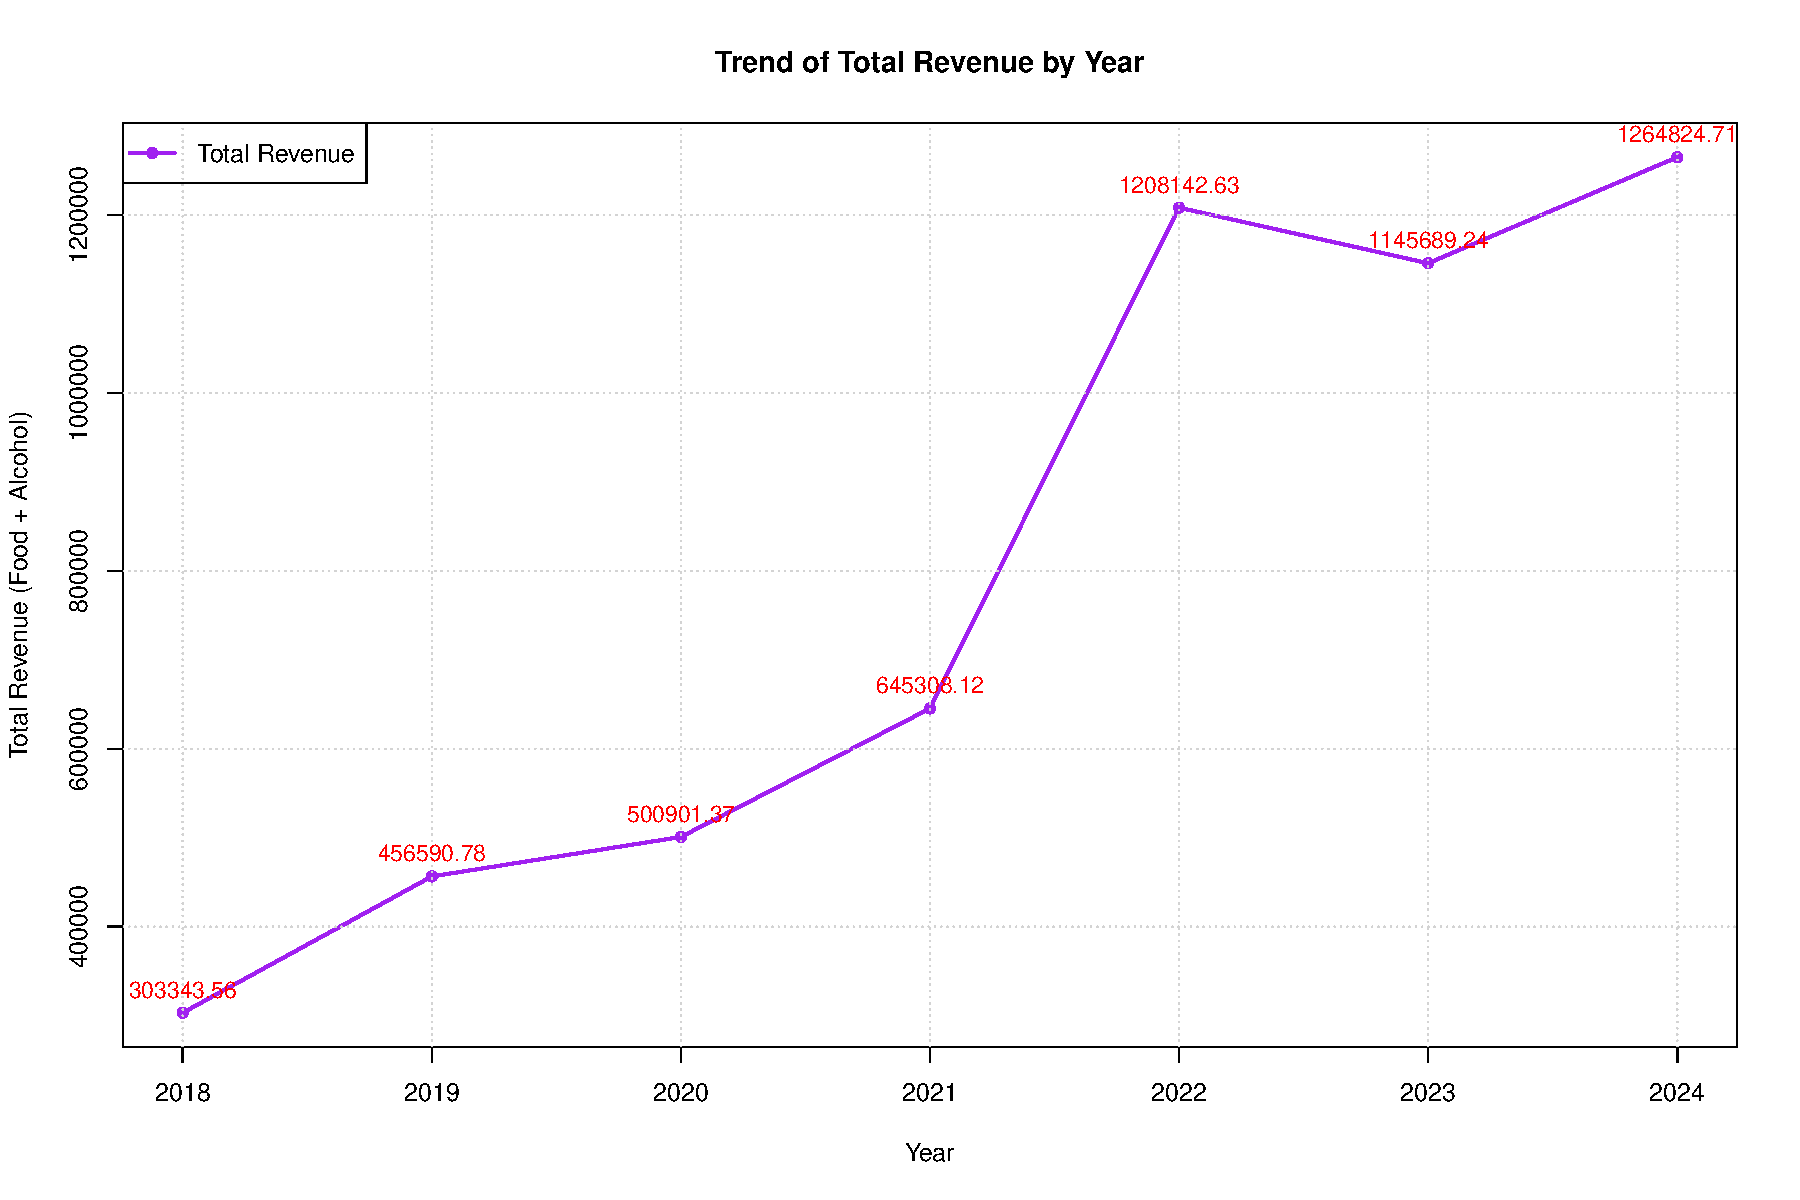
\includegraphics{RevenueReport.PractI.KrishnappaK_files/figure-latex/yearTrend-1.pdf}

\end{document}
